% Created by tikzDevice version 0.12.4 on 2023-06-17 14:01:25
% !TEX encoding = UTF-8 Unicode
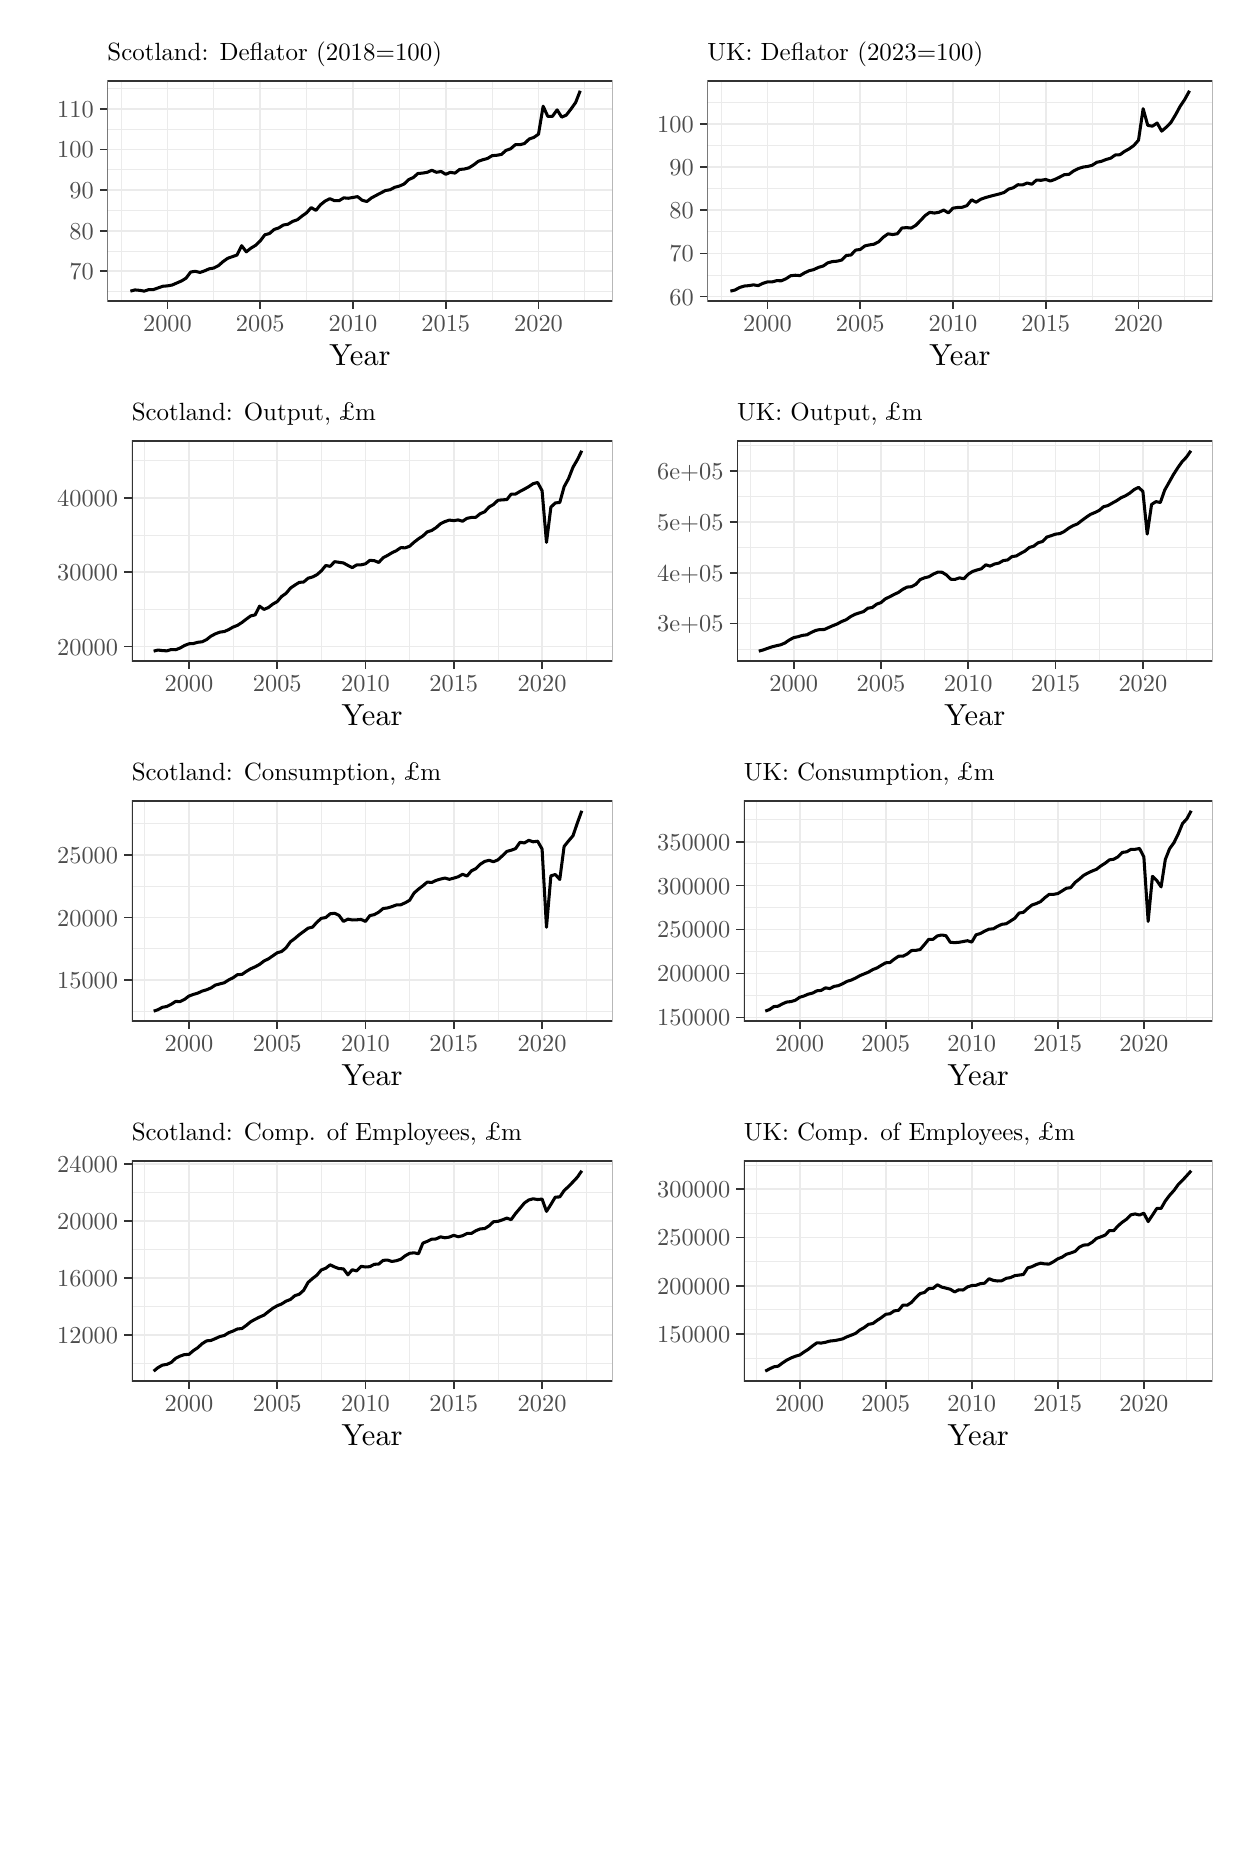
\begin{tikzpicture}[x=1pt,y=1pt]
\definecolor{fillColor}{RGB}{255,255,255}
\path[use as bounding box,fill=fillColor,fill opacity=0.00] (0,0) rectangle (433.62,650.43);
\begin{scope}
\path[clip] (  0.00,520.34) rectangle (216.81,650.43);
\definecolor{drawColor}{RGB}{255,255,255}
\definecolor{fillColor}{RGB}{255,255,255}

\path[draw=drawColor,line width= 0.6pt,line join=round,line cap=round,fill=fillColor] (  0.00,520.34) rectangle (216.81,650.43);
\end{scope}
\begin{scope}
\path[clip] ( 28.83,551.60) rectangle (211.31,631.24);
\definecolor{fillColor}{RGB}{255,255,255}

\path[fill=fillColor] ( 28.83,551.60) rectangle (211.31,631.24);
\definecolor{drawColor}{gray}{0.92}

\path[draw=drawColor,line width= 0.3pt,line join=round] ( 28.83,555.07) --
	(211.31,555.07);

\path[draw=drawColor,line width= 0.3pt,line join=round] ( 28.83,569.73) --
	(211.31,569.73);

\path[draw=drawColor,line width= 0.3pt,line join=round] ( 28.83,584.39) --
	(211.31,584.39);

\path[draw=drawColor,line width= 0.3pt,line join=round] ( 28.83,599.04) --
	(211.31,599.04);

\path[draw=drawColor,line width= 0.3pt,line join=round] ( 28.83,613.70) --
	(211.31,613.70);

\path[draw=drawColor,line width= 0.3pt,line join=round] ( 28.83,628.36) --
	(211.31,628.36);

\path[draw=drawColor,line width= 0.3pt,line join=round] ( 33.75,551.60) --
	( 33.75,631.24);

\path[draw=drawColor,line width= 0.3pt,line join=round] ( 67.28,551.60) --
	( 67.28,631.24);

\path[draw=drawColor,line width= 0.3pt,line join=round] (100.81,551.60) --
	(100.81,631.24);

\path[draw=drawColor,line width= 0.3pt,line join=round] (134.32,551.60) --
	(134.32,631.24);

\path[draw=drawColor,line width= 0.3pt,line join=round] (167.83,551.60) --
	(167.83,631.24);

\path[draw=drawColor,line width= 0.3pt,line join=round] (201.35,551.60) --
	(201.35,631.24);

\path[draw=drawColor,line width= 0.6pt,line join=round] ( 28.83,562.40) --
	(211.31,562.40);

\path[draw=drawColor,line width= 0.6pt,line join=round] ( 28.83,577.06) --
	(211.31,577.06);

\path[draw=drawColor,line width= 0.6pt,line join=round] ( 28.83,591.71) --
	(211.31,591.71);

\path[draw=drawColor,line width= 0.6pt,line join=round] ( 28.83,606.37) --
	(211.31,606.37);

\path[draw=drawColor,line width= 0.6pt,line join=round] ( 28.83,621.03) --
	(211.31,621.03);

\path[draw=drawColor,line width= 0.6pt,line join=round] ( 50.52,551.60) --
	( 50.52,631.24);

\path[draw=drawColor,line width= 0.6pt,line join=round] ( 84.05,551.60) --
	( 84.05,631.24);

\path[draw=drawColor,line width= 0.6pt,line join=round] (117.56,551.60) --
	(117.56,631.24);

\path[draw=drawColor,line width= 0.6pt,line join=round] (151.08,551.60) --
	(151.08,631.24);

\path[draw=drawColor,line width= 0.6pt,line join=round] (184.59,551.60) --
	(184.59,631.24);
\definecolor{drawColor}{RGB}{0,0,0}

\path[draw=drawColor,line width= 1.1pt,line join=round] ( 37.12,555.22) --
	( 38.77,555.66) --
	( 40.44,555.51) --
	( 42.13,555.22) --
	( 43.82,555.80) --
	( 45.47,555.80) --
	( 47.14,556.39) --
	( 48.83,556.98) --
	( 50.52,557.12) --
	( 52.19,557.42) --
	( 53.86,558.15) --
	( 55.55,558.88) --
	( 57.24,559.91) --
	( 58.89,562.11) --
	( 60.56,562.40) --
	( 62.25,561.96) --
	( 63.93,562.55) --
	( 65.59,563.28) --
	( 67.26,563.57) --
	( 68.95,564.45) --
	( 70.63,565.92) --
	( 72.29,567.09) --
	( 73.96,567.68) --
	( 75.64,568.26) --
	( 77.33,571.63) --
	( 79.00,569.43) --
	( 80.67,570.75) --
	( 82.36,571.78) --
	( 84.05,573.39) --
	( 85.70,575.59) --
	( 87.37,576.03) --
	( 89.06,577.50) --
	( 90.75,578.08) --
	( 92.40,579.11) --
	( 94.07,579.40) --
	( 95.76,580.43) --
	( 97.45,581.01) --
	( 99.10,582.33) --
	(100.77,583.51) --
	(102.46,585.41) --
	(104.15,584.39) --
	(105.82,586.44) --
	(107.49,587.76) --
	(109.18,588.64) --
	(110.86,587.90) --
	(112.52,587.90) --
	(114.19,588.93) --
	(115.87,588.78) --
	(117.56,589.08) --
	(119.21,589.37) --
	(120.88,588.05) --
	(122.57,587.61) --
	(124.26,588.93) --
	(125.91,589.81) --
	(127.58,590.69) --
	(129.27,591.57) --
	(130.96,591.86) --
	(132.63,592.74) --
	(134.30,593.18) --
	(135.99,593.91) --
	(137.68,595.52) --
	(139.33,596.26) --
	(141.00,597.72) --
	(142.69,597.87) --
	(144.38,598.16) --
	(146.03,598.90) --
	(147.70,598.16) --
	(149.39,598.46) --
	(151.08,597.43) --
	(152.73,598.16) --
	(154.40,597.87) --
	(156.09,599.19) --
	(157.77,599.34) --
	(159.44,599.78) --
	(161.11,600.80) --
	(162.80,602.12) --
	(164.49,602.71) --
	(166.14,603.15) --
	(167.81,604.17) --
	(169.50,604.32) --
	(171.19,604.61) --
	(172.84,606.08) --
	(174.51,606.66) --
	(176.20,608.13) --
	(177.89,608.13) --
	(179.54,608.57) --
	(181.21,610.18) --
	(182.90,610.77) --
	(184.59,611.94) --
	(186.26,622.05) --
	(187.93,618.39) --
	(189.62,618.39) --
	(191.31,620.73) --
	(192.96,618.10) --
	(194.63,618.83) --
	(196.32,621.03) --
	(198.00,623.37) --
	(199.66,627.62);
\definecolor{drawColor}{gray}{0.20}

\path[draw=drawColor,line width= 0.6pt,line join=round,line cap=round] ( 28.83,551.60) rectangle (211.31,631.24);
\end{scope}
\begin{scope}
\path[clip] (  0.00,  0.00) rectangle (433.62,650.43);
\definecolor{drawColor}{gray}{0.30}

\node[text=drawColor,anchor=base east,inner sep=0pt, outer sep=0pt, scale=  0.88] at ( 23.88,559.37) {70};

\node[text=drawColor,anchor=base east,inner sep=0pt, outer sep=0pt, scale=  0.88] at ( 23.88,574.03) {80};

\node[text=drawColor,anchor=base east,inner sep=0pt, outer sep=0pt, scale=  0.88] at ( 23.88,588.68) {90};

\node[text=drawColor,anchor=base east,inner sep=0pt, outer sep=0pt, scale=  0.88] at ( 23.88,603.34) {100};

\node[text=drawColor,anchor=base east,inner sep=0pt, outer sep=0pt, scale=  0.88] at ( 23.88,618.00) {110};
\end{scope}
\begin{scope}
\path[clip] (  0.00,  0.00) rectangle (433.62,650.43);
\definecolor{drawColor}{gray}{0.20}

\path[draw=drawColor,line width= 0.6pt,line join=round] ( 26.08,562.40) --
	( 28.83,562.40);

\path[draw=drawColor,line width= 0.6pt,line join=round] ( 26.08,577.06) --
	( 28.83,577.06);

\path[draw=drawColor,line width= 0.6pt,line join=round] ( 26.08,591.71) --
	( 28.83,591.71);

\path[draw=drawColor,line width= 0.6pt,line join=round] ( 26.08,606.37) --
	( 28.83,606.37);

\path[draw=drawColor,line width= 0.6pt,line join=round] ( 26.08,621.03) --
	( 28.83,621.03);
\end{scope}
\begin{scope}
\path[clip] (  0.00,  0.00) rectangle (433.62,650.43);
\definecolor{drawColor}{gray}{0.20}

\path[draw=drawColor,line width= 0.6pt,line join=round] ( 50.52,548.85) --
	( 50.52,551.60);

\path[draw=drawColor,line width= 0.6pt,line join=round] ( 84.05,548.85) --
	( 84.05,551.60);

\path[draw=drawColor,line width= 0.6pt,line join=round] (117.56,548.85) --
	(117.56,551.60);

\path[draw=drawColor,line width= 0.6pt,line join=round] (151.08,548.85) --
	(151.08,551.60);

\path[draw=drawColor,line width= 0.6pt,line join=round] (184.59,548.85) --
	(184.59,551.60);
\end{scope}
\begin{scope}
\path[clip] (  0.00,  0.00) rectangle (433.62,650.43);
\definecolor{drawColor}{gray}{0.30}

\node[text=drawColor,anchor=base,inner sep=0pt, outer sep=0pt, scale=  0.88] at ( 50.52,540.59) {2000};

\node[text=drawColor,anchor=base,inner sep=0pt, outer sep=0pt, scale=  0.88] at ( 84.05,540.59) {2005};

\node[text=drawColor,anchor=base,inner sep=0pt, outer sep=0pt, scale=  0.88] at (117.56,540.59) {2010};

\node[text=drawColor,anchor=base,inner sep=0pt, outer sep=0pt, scale=  0.88] at (151.08,540.59) {2015};

\node[text=drawColor,anchor=base,inner sep=0pt, outer sep=0pt, scale=  0.88] at (184.59,540.59) {2020};
\end{scope}
\begin{scope}
\path[clip] (  0.00,  0.00) rectangle (433.62,650.43);
\definecolor{drawColor}{RGB}{0,0,0}

\node[text=drawColor,anchor=base,inner sep=0pt, outer sep=0pt, scale=  1.10] at (120.07,528.27) {Year};
\end{scope}
\begin{scope}
\path[clip] (  0.00,  0.00) rectangle (433.62,650.43);
\definecolor{drawColor}{RGB}{0,0,0}

\node[text=drawColor,anchor=base west,inner sep=0pt, outer sep=0pt, scale=  0.90] at ( 28.83,638.73) {Scotland: Deflator (2018=100)};
\end{scope}
\begin{scope}
\path[clip] (216.81,520.34) rectangle (433.62,650.43);
\definecolor{drawColor}{RGB}{255,255,255}
\definecolor{fillColor}{RGB}{255,255,255}

\path[draw=drawColor,line width= 0.6pt,line join=round,line cap=round,fill=fillColor] (216.81,520.34) rectangle (433.62,650.43);
\end{scope}
\begin{scope}
\path[clip] (245.64,551.60) rectangle (428.12,631.24);
\definecolor{fillColor}{RGB}{255,255,255}

\path[fill=fillColor] (245.64,551.60) rectangle (428.12,631.24);
\definecolor{drawColor}{gray}{0.92}

\path[draw=drawColor,line width= 0.3pt,line join=round] (245.64,561.04) --
	(428.12,561.04);

\path[draw=drawColor,line width= 0.3pt,line join=round] (245.64,576.65) --
	(428.12,576.65);

\path[draw=drawColor,line width= 0.3pt,line join=round] (245.64,592.26) --
	(428.12,592.26);

\path[draw=drawColor,line width= 0.3pt,line join=round] (245.64,607.87) --
	(428.12,607.87);

\path[draw=drawColor,line width= 0.3pt,line join=round] (245.64,623.48) --
	(428.12,623.48);

\path[draw=drawColor,line width= 0.3pt,line join=round] (250.56,551.60) --
	(250.56,631.24);

\path[draw=drawColor,line width= 0.3pt,line join=round] (284.09,551.60) --
	(284.09,631.24);

\path[draw=drawColor,line width= 0.3pt,line join=round] (317.62,551.60) --
	(317.62,631.24);

\path[draw=drawColor,line width= 0.3pt,line join=round] (351.13,551.60) --
	(351.13,631.24);

\path[draw=drawColor,line width= 0.3pt,line join=round] (384.64,551.60) --
	(384.64,631.24);

\path[draw=drawColor,line width= 0.3pt,line join=round] (418.16,551.60) --
	(418.16,631.24);

\path[draw=drawColor,line width= 0.6pt,line join=round] (245.64,553.24) --
	(428.12,553.24);

\path[draw=drawColor,line width= 0.6pt,line join=round] (245.64,568.85) --
	(428.12,568.85);

\path[draw=drawColor,line width= 0.6pt,line join=round] (245.64,584.46) --
	(428.12,584.46);

\path[draw=drawColor,line width= 0.6pt,line join=round] (245.64,600.06) --
	(428.12,600.06);

\path[draw=drawColor,line width= 0.6pt,line join=round] (245.64,615.67) --
	(428.12,615.67);

\path[draw=drawColor,line width= 0.6pt,line join=round] (267.33,551.60) --
	(267.33,631.24);

\path[draw=drawColor,line width= 0.6pt,line join=round] (300.86,551.60) --
	(300.86,631.24);

\path[draw=drawColor,line width= 0.6pt,line join=round] (334.37,551.60) --
	(334.37,631.24);

\path[draw=drawColor,line width= 0.6pt,line join=round] (367.89,551.60) --
	(367.89,631.24);

\path[draw=drawColor,line width= 0.6pt,line join=round] (401.40,551.60) --
	(401.40,631.24);
\definecolor{drawColor}{RGB}{0,0,0}

\path[draw=drawColor,line width= 1.1pt,line join=round] (253.93,555.22) --
	(255.58,555.62) --
	(257.25,556.53) --
	(258.94,557.06) --
	(260.63,557.21) --
	(262.28,557.49) --
	(263.95,557.22) --
	(265.64,558.02) --
	(267.33,558.57) --
	(269.00,558.57) --
	(270.67,559.00) --
	(272.36,558.96) --
	(274.05,559.72) --
	(275.70,560.78) --
	(277.37,560.97) --
	(279.06,560.83) --
	(280.74,561.84) --
	(282.40,562.60) --
	(284.07,563.01) --
	(285.76,563.81) --
	(287.44,564.29) --
	(289.10,565.43) --
	(290.77,565.90) --
	(292.45,566.04) --
	(294.14,566.46) --
	(295.81,568.11) --
	(297.48,568.27) --
	(299.17,570.05) --
	(300.86,570.28) --
	(302.51,571.56) --
	(304.18,571.93) --
	(305.87,572.20) --
	(307.56,573.10) --
	(309.21,574.73) --
	(310.88,575.93) --
	(312.57,575.67) --
	(314.26,575.95) --
	(315.91,578.03) --
	(317.58,578.17) --
	(319.27,578.02) --
	(320.96,579.03) --
	(322.63,580.73) --
	(324.30,582.54) --
	(325.99,583.70) --
	(327.67,583.43) --
	(329.33,583.73) --
	(331.00,584.52) --
	(332.68,583.51) --
	(334.37,585.22) --
	(336.02,585.45) --
	(337.69,585.53) --
	(339.38,586.11) --
	(341.07,588.22) --
	(342.72,587.35) --
	(344.39,588.42) --
	(346.08,589.02) --
	(347.77,589.49) --
	(349.44,589.93) --
	(351.11,590.34) --
	(352.80,590.86) --
	(354.49,592.10) --
	(356.14,592.57) --
	(357.81,593.67) --
	(359.50,593.60) --
	(361.19,594.30) --
	(362.84,593.84) --
	(364.51,595.35) --
	(366.20,595.27) --
	(367.89,595.58) --
	(369.54,595.00) --
	(371.21,595.62) --
	(372.90,596.42) --
	(374.58,597.31) --
	(376.25,597.41) --
	(377.92,598.63) --
	(379.61,599.48) --
	(381.30,600.04) --
	(382.95,600.27) --
	(384.62,600.68) --
	(386.31,601.78) --
	(388.00,602.13) --
	(389.65,602.78) --
	(391.32,603.26) --
	(393.01,604.41) --
	(394.70,604.52) --
	(396.35,605.72) --
	(398.02,606.63) --
	(399.71,607.85) --
	(401.40,609.78) --
	(403.07,621.14) --
	(404.74,615.11) --
	(406.43,614.83) --
	(408.12,615.97) --
	(409.77,613.03) --
	(411.44,614.46) --
	(413.13,616.20) --
	(414.81,619.00) --
	(416.47,622.06) --
	(418.14,624.56) --
	(419.83,627.62);
\definecolor{drawColor}{gray}{0.20}

\path[draw=drawColor,line width= 0.6pt,line join=round,line cap=round] (245.64,551.60) rectangle (428.12,631.24);
\end{scope}
\begin{scope}
\path[clip] (  0.00,  0.00) rectangle (433.62,650.43);
\definecolor{drawColor}{gray}{0.30}

\node[text=drawColor,anchor=base east,inner sep=0pt, outer sep=0pt, scale=  0.88] at (240.69,550.21) {60};

\node[text=drawColor,anchor=base east,inner sep=0pt, outer sep=0pt, scale=  0.88] at (240.69,565.82) {70};

\node[text=drawColor,anchor=base east,inner sep=0pt, outer sep=0pt, scale=  0.88] at (240.69,581.42) {80};

\node[text=drawColor,anchor=base east,inner sep=0pt, outer sep=0pt, scale=  0.88] at (240.69,597.03) {90};

\node[text=drawColor,anchor=base east,inner sep=0pt, outer sep=0pt, scale=  0.88] at (240.69,612.64) {100};
\end{scope}
\begin{scope}
\path[clip] (  0.00,  0.00) rectangle (433.62,650.43);
\definecolor{drawColor}{gray}{0.20}

\path[draw=drawColor,line width= 0.6pt,line join=round] (242.89,553.24) --
	(245.64,553.24);

\path[draw=drawColor,line width= 0.6pt,line join=round] (242.89,568.85) --
	(245.64,568.85);

\path[draw=drawColor,line width= 0.6pt,line join=round] (242.89,584.46) --
	(245.64,584.46);

\path[draw=drawColor,line width= 0.6pt,line join=round] (242.89,600.06) --
	(245.64,600.06);

\path[draw=drawColor,line width= 0.6pt,line join=round] (242.89,615.67) --
	(245.64,615.67);
\end{scope}
\begin{scope}
\path[clip] (  0.00,  0.00) rectangle (433.62,650.43);
\definecolor{drawColor}{gray}{0.20}

\path[draw=drawColor,line width= 0.6pt,line join=round] (267.33,548.85) --
	(267.33,551.60);

\path[draw=drawColor,line width= 0.6pt,line join=round] (300.86,548.85) --
	(300.86,551.60);

\path[draw=drawColor,line width= 0.6pt,line join=round] (334.37,548.85) --
	(334.37,551.60);

\path[draw=drawColor,line width= 0.6pt,line join=round] (367.89,548.85) --
	(367.89,551.60);

\path[draw=drawColor,line width= 0.6pt,line join=round] (401.40,548.85) --
	(401.40,551.60);
\end{scope}
\begin{scope}
\path[clip] (  0.00,  0.00) rectangle (433.62,650.43);
\definecolor{drawColor}{gray}{0.30}

\node[text=drawColor,anchor=base,inner sep=0pt, outer sep=0pt, scale=  0.88] at (267.33,540.59) {2000};

\node[text=drawColor,anchor=base,inner sep=0pt, outer sep=0pt, scale=  0.88] at (300.86,540.59) {2005};

\node[text=drawColor,anchor=base,inner sep=0pt, outer sep=0pt, scale=  0.88] at (334.37,540.59) {2010};

\node[text=drawColor,anchor=base,inner sep=0pt, outer sep=0pt, scale=  0.88] at (367.89,540.59) {2015};

\node[text=drawColor,anchor=base,inner sep=0pt, outer sep=0pt, scale=  0.88] at (401.40,540.59) {2020};
\end{scope}
\begin{scope}
\path[clip] (  0.00,  0.00) rectangle (433.62,650.43);
\definecolor{drawColor}{RGB}{0,0,0}

\node[text=drawColor,anchor=base,inner sep=0pt, outer sep=0pt, scale=  1.10] at (336.88,528.27) {Year};
\end{scope}
\begin{scope}
\path[clip] (  0.00,  0.00) rectangle (433.62,650.43);
\definecolor{drawColor}{RGB}{0,0,0}

\node[text=drawColor,anchor=base west,inner sep=0pt, outer sep=0pt, scale=  0.90] at (245.64,638.73) {UK: Deflator (2023=100)};
\end{scope}
\begin{scope}
\path[clip] (  0.00,390.26) rectangle (216.81,520.34);
\definecolor{drawColor}{RGB}{255,255,255}
\definecolor{fillColor}{RGB}{255,255,255}

\path[draw=drawColor,line width= 0.6pt,line join=round,line cap=round,fill=fillColor] (  0.00,390.26) rectangle (216.81,520.34);
\end{scope}
\begin{scope}
\path[clip] ( 37.62,421.51) rectangle (211.31,501.16);
\definecolor{fillColor}{RGB}{255,255,255}

\path[fill=fillColor] ( 37.62,421.51) rectangle (211.31,501.16);
\definecolor{drawColor}{gray}{0.92}

\path[draw=drawColor,line width= 0.3pt,line join=round] ( 37.62,440.20) --
	(211.31,440.20);

\path[draw=drawColor,line width= 0.3pt,line join=round] ( 37.62,467.08) --
	(211.31,467.08);

\path[draw=drawColor,line width= 0.3pt,line join=round] ( 37.62,493.95) --
	(211.31,493.95);

\path[draw=drawColor,line width= 0.3pt,line join=round] ( 42.31,421.51) --
	( 42.31,501.16);

\path[draw=drawColor,line width= 0.3pt,line join=round] ( 74.23,421.51) --
	( 74.23,501.16);

\path[draw=drawColor,line width= 0.3pt,line join=round] (106.13,421.51) --
	(106.13,501.16);

\path[draw=drawColor,line width= 0.3pt,line join=round] (138.03,421.51) --
	(138.03,501.16);

\path[draw=drawColor,line width= 0.3pt,line join=round] (169.93,421.51) --
	(169.93,501.16);

\path[draw=drawColor,line width= 0.3pt,line join=round] (201.83,421.51) --
	(201.83,501.16);

\path[draw=drawColor,line width= 0.6pt,line join=round] ( 37.62,426.76) --
	(211.31,426.76);

\path[draw=drawColor,line width= 0.6pt,line join=round] ( 37.62,453.64) --
	(211.31,453.64);

\path[draw=drawColor,line width= 0.6pt,line join=round] ( 37.62,480.52) --
	(211.31,480.52);

\path[draw=drawColor,line width= 0.6pt,line join=round] ( 58.27,421.51) --
	( 58.27,501.16);

\path[draw=drawColor,line width= 0.6pt,line join=round] ( 90.19,421.51) --
	( 90.19,501.16);

\path[draw=drawColor,line width= 0.6pt,line join=round] (122.08,421.51) --
	(122.08,501.16);

\path[draw=drawColor,line width= 0.6pt,line join=round] (153.98,421.51) --
	(153.98,501.16);

\path[draw=drawColor,line width= 0.6pt,line join=round] (185.88,421.51) --
	(185.88,501.16);
\definecolor{drawColor}{RGB}{0,0,0}

\path[draw=drawColor,line width= 1.1pt,line join=round] ( 45.52,425.13) --
	( 47.09,425.54) --
	( 48.68,425.33) --
	( 50.29,425.24) --
	( 51.89,425.72) --
	( 53.47,425.64) --
	( 55.06,426.25) --
	( 56.66,427.16) --
	( 58.27,427.79) --
	( 59.86,427.88) --
	( 61.45,428.33) --
	( 63.06,428.52) --
	( 64.66,429.32) --
	( 66.24,430.56) --
	( 67.83,431.39) --
	( 69.43,432.00) --
	( 71.04,432.22) --
	( 72.61,432.90) --
	( 74.20,433.82) --
	( 75.81,434.45) --
	( 77.42,435.49) --
	( 78.99,436.70) --
	( 80.58,437.86) --
	( 82.18,438.23) --
	( 83.79,441.39) --
	( 85.38,440.21) --
	( 86.97,440.89) --
	( 88.58,442.13) --
	( 90.19,443.05) --
	( 91.76,444.89) --
	( 93.35,446.00) --
	( 94.95,447.90) --
	( 96.56,449.01) --
	( 98.13,449.98) --
	( 99.72,450.11) --
	(101.33,451.48) --
	(102.94,451.94) --
	(104.51,452.75) --
	(106.10,454.13) --
	(107.71,456.08) --
	(109.31,455.77) --
	(110.90,457.46) --
	(112.49,457.24) --
	(114.10,457.01) --
	(115.71,456.11) --
	(117.28,455.30) --
	(118.87,456.28) --
	(120.48,456.32) --
	(122.08,456.69) --
	(123.65,457.94) --
	(125.24,457.83) --
	(126.85,457.18) --
	(128.46,458.90) --
	(130.03,459.72) --
	(131.62,460.68) --
	(133.23,461.44) --
	(134.83,462.52) --
	(136.42,462.47) --
	(138.01,463.04) --
	(139.62,464.49) --
	(141.23,465.73) --
	(142.80,466.76) --
	(144.39,468.23) --
	(146.00,468.74) --
	(147.60,469.78) --
	(149.18,471.17) --
	(150.77,471.94) --
	(152.37,472.49) --
	(153.98,472.28) --
	(155.55,472.55) --
	(157.14,472.07) --
	(158.75,473.13) --
	(160.36,473.45) --
	(161.95,473.50) --
	(163.53,474.81) --
	(165.14,475.49) --
	(166.75,477.24) --
	(168.32,478.12) --
	(169.91,479.64) --
	(171.52,479.81) --
	(173.13,479.88) --
	(174.70,481.85) --
	(176.29,481.88) --
	(177.89,482.86) --
	(179.50,483.69) --
	(181.07,484.59) --
	(182.66,485.65) --
	(184.27,486.08) --
	(185.88,483.11) --
	(187.47,464.43) --
	(189.06,477.16) --
	(190.66,478.70) --
	(192.27,478.84) --
	(193.84,484.53) --
	(195.43,487.44) --
	(197.04,491.57) --
	(198.65,494.34) --
	(200.22,497.54);
\definecolor{drawColor}{gray}{0.20}

\path[draw=drawColor,line width= 0.6pt,line join=round,line cap=round] ( 37.62,421.51) rectangle (211.31,501.16);
\end{scope}
\begin{scope}
\path[clip] (  0.00,  0.00) rectangle (433.62,650.43);
\definecolor{drawColor}{gray}{0.30}

\node[text=drawColor,anchor=base east,inner sep=0pt, outer sep=0pt, scale=  0.88] at ( 32.67,423.73) {20000};

\node[text=drawColor,anchor=base east,inner sep=0pt, outer sep=0pt, scale=  0.88] at ( 32.67,450.61) {30000};

\node[text=drawColor,anchor=base east,inner sep=0pt, outer sep=0pt, scale=  0.88] at ( 32.67,477.49) {40000};
\end{scope}
\begin{scope}
\path[clip] (  0.00,  0.00) rectangle (433.62,650.43);
\definecolor{drawColor}{gray}{0.20}

\path[draw=drawColor,line width= 0.6pt,line join=round] ( 34.87,426.76) --
	( 37.62,426.76);

\path[draw=drawColor,line width= 0.6pt,line join=round] ( 34.87,453.64) --
	( 37.62,453.64);

\path[draw=drawColor,line width= 0.6pt,line join=round] ( 34.87,480.52) --
	( 37.62,480.52);
\end{scope}
\begin{scope}
\path[clip] (  0.00,  0.00) rectangle (433.62,650.43);
\definecolor{drawColor}{gray}{0.20}

\path[draw=drawColor,line width= 0.6pt,line join=round] ( 58.27,418.76) --
	( 58.27,421.51);

\path[draw=drawColor,line width= 0.6pt,line join=round] ( 90.19,418.76) --
	( 90.19,421.51);

\path[draw=drawColor,line width= 0.6pt,line join=round] (122.08,418.76) --
	(122.08,421.51);

\path[draw=drawColor,line width= 0.6pt,line join=round] (153.98,418.76) --
	(153.98,421.51);

\path[draw=drawColor,line width= 0.6pt,line join=round] (185.88,418.76) --
	(185.88,421.51);
\end{scope}
\begin{scope}
\path[clip] (  0.00,  0.00) rectangle (433.62,650.43);
\definecolor{drawColor}{gray}{0.30}

\node[text=drawColor,anchor=base,inner sep=0pt, outer sep=0pt, scale=  0.88] at ( 58.27,410.50) {2000};

\node[text=drawColor,anchor=base,inner sep=0pt, outer sep=0pt, scale=  0.88] at ( 90.19,410.50) {2005};

\node[text=drawColor,anchor=base,inner sep=0pt, outer sep=0pt, scale=  0.88] at (122.08,410.50) {2010};

\node[text=drawColor,anchor=base,inner sep=0pt, outer sep=0pt, scale=  0.88] at (153.98,410.50) {2015};

\node[text=drawColor,anchor=base,inner sep=0pt, outer sep=0pt, scale=  0.88] at (185.88,410.50) {2020};
\end{scope}
\begin{scope}
\path[clip] (  0.00,  0.00) rectangle (433.62,650.43);
\definecolor{drawColor}{RGB}{0,0,0}

\node[text=drawColor,anchor=base,inner sep=0pt, outer sep=0pt, scale=  1.10] at (124.47,398.19) {Year};
\end{scope}
\begin{scope}
\path[clip] (  0.00,  0.00) rectangle (433.62,650.43);
\definecolor{drawColor}{RGB}{0,0,0}

\node[text=drawColor,anchor=base west,inner sep=0pt, outer sep=0pt, scale=  0.90] at ( 37.62,508.65) {Scotland: Output, £m};
\end{scope}
\begin{scope}
\path[clip] (216.81,390.26) rectangle (433.62,520.34);
\definecolor{drawColor}{RGB}{255,255,255}
\definecolor{fillColor}{RGB}{255,255,255}

\path[draw=drawColor,line width= 0.6pt,line join=round,line cap=round,fill=fillColor] (216.81,390.26) rectangle (433.62,520.34);
\end{scope}
\begin{scope}
\path[clip] (256.39,421.51) rectangle (428.12,501.16);
\definecolor{fillColor}{RGB}{255,255,255}

\path[fill=fillColor] (256.39,421.51) rectangle (428.12,501.16);
\definecolor{drawColor}{gray}{0.92}

\path[draw=drawColor,line width= 0.3pt,line join=round] (256.39,425.91) --
	(428.12,425.91);

\path[draw=drawColor,line width= 0.3pt,line join=round] (256.39,444.29) --
	(428.12,444.29);

\path[draw=drawColor,line width= 0.3pt,line join=round] (256.39,462.68) --
	(428.12,462.68);

\path[draw=drawColor,line width= 0.3pt,line join=round] (256.39,481.06) --
	(428.12,481.06);

\path[draw=drawColor,line width= 0.3pt,line join=round] (256.39,499.45) --
	(428.12,499.45);

\path[draw=drawColor,line width= 0.3pt,line join=round] (261.03,421.51) --
	(261.03,501.16);

\path[draw=drawColor,line width= 0.3pt,line join=round] (292.58,421.51) --
	(292.58,501.16);

\path[draw=drawColor,line width= 0.3pt,line join=round] (324.13,421.51) --
	(324.13,501.16);

\path[draw=drawColor,line width= 0.3pt,line join=round] (355.67,421.51) --
	(355.67,501.16);

\path[draw=drawColor,line width= 0.3pt,line join=round] (387.20,421.51) --
	(387.20,501.16);

\path[draw=drawColor,line width= 0.3pt,line join=round] (418.75,421.51) --
	(418.75,501.16);

\path[draw=drawColor,line width= 0.6pt,line join=round] (256.39,435.10) --
	(428.12,435.10);

\path[draw=drawColor,line width= 0.6pt,line join=round] (256.39,453.48) --
	(428.12,453.48);

\path[draw=drawColor,line width= 0.6pt,line join=round] (256.39,471.87) --
	(428.12,471.87);

\path[draw=drawColor,line width= 0.6pt,line join=round] (256.39,490.25) --
	(428.12,490.25);

\path[draw=drawColor,line width= 0.6pt,line join=round] (276.80,421.51) --
	(276.80,501.16);

\path[draw=drawColor,line width= 0.6pt,line join=round] (308.36,421.51) --
	(308.36,501.16);

\path[draw=drawColor,line width= 0.6pt,line join=round] (339.90,421.51) --
	(339.90,501.16);

\path[draw=drawColor,line width= 0.6pt,line join=round] (371.44,421.51) --
	(371.44,501.16);

\path[draw=drawColor,line width= 0.6pt,line join=round] (402.97,421.51) --
	(402.97,501.16);
\definecolor{drawColor}{RGB}{0,0,0}

\path[draw=drawColor,line width= 1.1pt,line join=round] (264.19,425.13) --
	(265.75,425.56) --
	(267.32,426.13) --
	(268.91,426.68) --
	(270.50,427.08) --
	(272.05,427.41) --
	(273.63,428.08) --
	(275.21,429.17) --
	(276.80,430.02) --
	(278.37,430.35) --
	(279.95,430.83) --
	(281.54,431.03) --
	(283.12,431.86) --
	(284.68,432.60) --
	(286.25,432.94) --
	(287.84,432.95) --
	(289.43,433.67) --
	(290.98,434.35) --
	(292.56,434.97) --
	(294.14,435.85) --
	(295.73,436.47) --
	(297.29,437.57) --
	(298.86,438.40) --
	(300.45,438.93) --
	(302.04,439.43) --
	(303.61,440.66) --
	(305.18,440.90) --
	(306.77,442.10) --
	(308.36,442.69) --
	(309.91,444.02) --
	(311.48,444.78) --
	(313.07,445.61) --
	(314.66,446.37) --
	(316.22,447.48) --
	(317.79,448.28) --
	(319.38,448.43) --
	(320.97,449.31) --
	(322.52,451.01) --
	(324.09,451.64) --
	(325.68,452.02) --
	(327.27,452.98) --
	(328.84,453.67) --
	(330.41,453.64) --
	(332.00,452.67) --
	(333.59,451.11) --
	(335.15,451.08) --
	(336.72,451.62) --
	(338.31,451.29) --
	(339.90,452.96) --
	(341.45,453.92) --
	(343.02,454.45) --
	(344.61,454.89) --
	(346.20,456.33) --
	(347.76,455.86) --
	(349.33,456.61) --
	(350.92,456.94) --
	(352.51,457.85) --
	(354.08,458.08) --
	(355.65,459.29) --
	(357.24,459.53) --
	(358.83,460.47) --
	(360.38,461.30) --
	(361.95,462.59) --
	(363.54,463.08) --
	(365.13,464.30) --
	(366.69,464.75) --
	(368.26,466.35) --
	(369.85,466.86) --
	(371.44,467.42) --
	(372.99,467.60) --
	(374.56,468.38) --
	(376.15,469.56) --
	(377.74,470.47) --
	(379.31,471.10) --
	(380.88,472.32) --
	(382.47,473.49) --
	(384.06,474.56) --
	(385.62,475.22) --
	(387.19,475.99) --
	(388.78,477.34) --
	(390.36,477.73) --
	(391.92,478.63) --
	(393.49,479.50) --
	(395.08,480.56) --
	(396.67,481.27) --
	(398.22,482.22) --
	(399.80,483.49) --
	(401.38,484.32) --
	(402.97,482.88) --
	(404.54,467.43) --
	(406.12,478.15) --
	(407.71,479.16) --
	(409.29,478.84) --
	(410.85,483.31) --
	(412.42,486.09) --
	(414.01,488.92) --
	(415.60,491.41) --
	(417.15,493.60) --
	(418.73,495.25) --
	(420.31,497.54);
\definecolor{drawColor}{gray}{0.20}

\path[draw=drawColor,line width= 0.6pt,line join=round,line cap=round] (256.39,421.51) rectangle (428.12,501.16);
\end{scope}
\begin{scope}
\path[clip] (  0.00,  0.00) rectangle (433.62,650.43);
\definecolor{drawColor}{gray}{0.30}

\node[text=drawColor,anchor=base east,inner sep=0pt, outer sep=0pt, scale=  0.88] at (251.44,432.07) {3e+05};

\node[text=drawColor,anchor=base east,inner sep=0pt, outer sep=0pt, scale=  0.88] at (251.44,450.45) {4e+05};

\node[text=drawColor,anchor=base east,inner sep=0pt, outer sep=0pt, scale=  0.88] at (251.44,468.84) {5e+05};

\node[text=drawColor,anchor=base east,inner sep=0pt, outer sep=0pt, scale=  0.88] at (251.44,487.22) {6e+05};
\end{scope}
\begin{scope}
\path[clip] (  0.00,  0.00) rectangle (433.62,650.43);
\definecolor{drawColor}{gray}{0.20}

\path[draw=drawColor,line width= 0.6pt,line join=round] (253.64,435.10) --
	(256.39,435.10);

\path[draw=drawColor,line width= 0.6pt,line join=round] (253.64,453.48) --
	(256.39,453.48);

\path[draw=drawColor,line width= 0.6pt,line join=round] (253.64,471.87) --
	(256.39,471.87);

\path[draw=drawColor,line width= 0.6pt,line join=round] (253.64,490.25) --
	(256.39,490.25);
\end{scope}
\begin{scope}
\path[clip] (  0.00,  0.00) rectangle (433.62,650.43);
\definecolor{drawColor}{gray}{0.20}

\path[draw=drawColor,line width= 0.6pt,line join=round] (276.80,418.76) --
	(276.80,421.51);

\path[draw=drawColor,line width= 0.6pt,line join=round] (308.36,418.76) --
	(308.36,421.51);

\path[draw=drawColor,line width= 0.6pt,line join=round] (339.90,418.76) --
	(339.90,421.51);

\path[draw=drawColor,line width= 0.6pt,line join=round] (371.44,418.76) --
	(371.44,421.51);

\path[draw=drawColor,line width= 0.6pt,line join=round] (402.97,418.76) --
	(402.97,421.51);
\end{scope}
\begin{scope}
\path[clip] (  0.00,  0.00) rectangle (433.62,650.43);
\definecolor{drawColor}{gray}{0.30}

\node[text=drawColor,anchor=base,inner sep=0pt, outer sep=0pt, scale=  0.88] at (276.80,410.50) {2000};

\node[text=drawColor,anchor=base,inner sep=0pt, outer sep=0pt, scale=  0.88] at (308.36,410.50) {2005};

\node[text=drawColor,anchor=base,inner sep=0pt, outer sep=0pt, scale=  0.88] at (339.90,410.50) {2010};

\node[text=drawColor,anchor=base,inner sep=0pt, outer sep=0pt, scale=  0.88] at (371.44,410.50) {2015};

\node[text=drawColor,anchor=base,inner sep=0pt, outer sep=0pt, scale=  0.88] at (402.97,410.50) {2020};
\end{scope}
\begin{scope}
\path[clip] (  0.00,  0.00) rectangle (433.62,650.43);
\definecolor{drawColor}{RGB}{0,0,0}

\node[text=drawColor,anchor=base,inner sep=0pt, outer sep=0pt, scale=  1.10] at (342.25,398.19) {Year};
\end{scope}
\begin{scope}
\path[clip] (  0.00,  0.00) rectangle (433.62,650.43);
\definecolor{drawColor}{RGB}{0,0,0}

\node[text=drawColor,anchor=base west,inner sep=0pt, outer sep=0pt, scale=  0.90] at (256.39,508.65) {UK: Output, £m};
\end{scope}
\begin{scope}
\path[clip] (  0.00,260.17) rectangle (216.81,390.26);
\definecolor{drawColor}{RGB}{255,255,255}
\definecolor{fillColor}{RGB}{255,255,255}

\path[draw=drawColor,line width= 0.6pt,line join=round,line cap=round,fill=fillColor] (  0.00,260.17) rectangle (216.81,390.26);
\end{scope}
\begin{scope}
\path[clip] ( 37.62,291.43) rectangle (211.31,371.07);
\definecolor{fillColor}{RGB}{255,255,255}

\path[fill=fillColor] ( 37.62,291.43) rectangle (211.31,371.07);
\definecolor{drawColor}{gray}{0.92}

\path[draw=drawColor,line width= 0.3pt,line join=round] ( 37.62,294.96) --
	(211.31,294.96);

\path[draw=drawColor,line width= 0.3pt,line join=round] ( 37.62,317.54) --
	(211.31,317.54);

\path[draw=drawColor,line width= 0.3pt,line join=round] ( 37.62,340.13) --
	(211.31,340.13);

\path[draw=drawColor,line width= 0.3pt,line join=round] ( 37.62,362.71) --
	(211.31,362.71);

\path[draw=drawColor,line width= 0.3pt,line join=round] ( 42.31,291.43) --
	( 42.31,371.07);

\path[draw=drawColor,line width= 0.3pt,line join=round] ( 74.23,291.43) --
	( 74.23,371.07);

\path[draw=drawColor,line width= 0.3pt,line join=round] (106.13,291.43) --
	(106.13,371.07);

\path[draw=drawColor,line width= 0.3pt,line join=round] (138.03,291.43) --
	(138.03,371.07);

\path[draw=drawColor,line width= 0.3pt,line join=round] (169.93,291.43) --
	(169.93,371.07);

\path[draw=drawColor,line width= 0.3pt,line join=round] (201.83,291.43) --
	(201.83,371.07);

\path[draw=drawColor,line width= 0.6pt,line join=round] ( 37.62,306.25) --
	(211.31,306.25);

\path[draw=drawColor,line width= 0.6pt,line join=round] ( 37.62,328.83) --
	(211.31,328.83);

\path[draw=drawColor,line width= 0.6pt,line join=round] ( 37.62,351.42) --
	(211.31,351.42);

\path[draw=drawColor,line width= 0.6pt,line join=round] ( 58.27,291.43) --
	( 58.27,371.07);

\path[draw=drawColor,line width= 0.6pt,line join=round] ( 90.19,291.43) --
	( 90.19,371.07);

\path[draw=drawColor,line width= 0.6pt,line join=round] (122.08,291.43) --
	(122.08,371.07);

\path[draw=drawColor,line width= 0.6pt,line join=round] (153.98,291.43) --
	(153.98,371.07);

\path[draw=drawColor,line width= 0.6pt,line join=round] (185.88,291.43) --
	(185.88,371.07);
\definecolor{drawColor}{RGB}{0,0,0}

\path[draw=drawColor,line width= 1.1pt,line join=round] ( 45.52,295.05) --
	( 47.09,295.57) --
	( 48.68,296.44) --
	( 50.29,296.73) --
	( 51.89,297.55) --
	( 53.47,298.56) --
	( 55.06,298.49) --
	( 56.66,299.28) --
	( 58.27,300.50) --
	( 59.86,301.09) --
	( 61.45,301.55) --
	( 63.06,302.30) --
	( 64.66,302.77) --
	( 66.24,303.43) --
	( 67.83,304.47) --
	( 69.43,304.89) --
	( 71.04,305.30) --
	( 72.61,306.32) --
	( 74.20,307.09) --
	( 75.81,308.24) --
	( 77.42,308.32) --
	( 78.99,309.39) --
	( 80.58,310.35) --
	( 82.18,311.06) --
	( 83.79,311.94) --
	( 85.38,313.15) --
	( 86.97,313.93) --
	( 88.58,315.04) --
	( 90.19,316.15) --
	( 91.76,316.60) --
	( 93.35,317.92) --
	( 94.95,320.12) --
	( 96.56,321.32) --
	( 98.13,322.66) --
	( 99.72,323.83) --
	(101.33,325.02) --
	(102.94,325.41) --
	(104.51,327.17) --
	(106.10,328.58) --
	(107.71,328.87) --
	(109.31,330.23) --
	(110.90,330.42) --
	(112.49,329.67) --
	(114.10,327.47) --
	(115.71,328.30) --
	(117.28,327.99) --
	(118.87,328.05) --
	(120.48,328.18) --
	(122.08,327.47) --
	(123.65,329.58) --
	(125.24,329.92) --
	(126.85,330.82) --
	(128.46,332.14) --
	(130.03,332.34) --
	(131.62,332.82) --
	(133.23,333.42) --
	(134.83,333.49) --
	(136.42,334.21) --
	(138.01,335.10) --
	(139.62,337.73) --
	(141.23,339.14) --
	(142.80,340.35) --
	(144.39,341.69) --
	(146.00,341.54) --
	(147.60,342.30) --
	(149.18,342.77) --
	(150.77,343.14) --
	(152.37,342.68) --
	(153.98,343.12) --
	(155.55,343.60) --
	(157.14,344.50) --
	(158.75,343.87) --
	(160.36,345.75) --
	(161.95,346.54) --
	(163.53,348.11) --
	(165.14,349.15) --
	(166.75,349.55) --
	(168.32,349.04) --
	(169.91,349.70) --
	(171.52,351.17) --
	(173.13,352.77) --
	(174.70,353.19) --
	(176.29,353.77) --
	(177.89,356.05) --
	(179.50,355.84) --
	(181.07,356.77) --
	(182.66,356.24) --
	(184.27,356.45) --
	(185.88,353.64) --
	(187.47,325.37) --
	(189.06,343.94) --
	(190.66,344.42) --
	(192.27,342.63) --
	(193.84,354.56) --
	(195.43,356.54) --
	(197.04,358.42) --
	(198.65,363.11) --
	(200.22,367.45);
\definecolor{drawColor}{gray}{0.20}

\path[draw=drawColor,line width= 0.6pt,line join=round,line cap=round] ( 37.62,291.43) rectangle (211.31,371.07);
\end{scope}
\begin{scope}
\path[clip] (  0.00,  0.00) rectangle (433.62,650.43);
\definecolor{drawColor}{gray}{0.30}

\node[text=drawColor,anchor=base east,inner sep=0pt, outer sep=0pt, scale=  0.88] at ( 32.67,303.22) {15000};

\node[text=drawColor,anchor=base east,inner sep=0pt, outer sep=0pt, scale=  0.88] at ( 32.67,325.80) {20000};

\node[text=drawColor,anchor=base east,inner sep=0pt, outer sep=0pt, scale=  0.88] at ( 32.67,348.39) {25000};
\end{scope}
\begin{scope}
\path[clip] (  0.00,  0.00) rectangle (433.62,650.43);
\definecolor{drawColor}{gray}{0.20}

\path[draw=drawColor,line width= 0.6pt,line join=round] ( 34.87,306.25) --
	( 37.62,306.25);

\path[draw=drawColor,line width= 0.6pt,line join=round] ( 34.87,328.83) --
	( 37.62,328.83);

\path[draw=drawColor,line width= 0.6pt,line join=round] ( 34.87,351.42) --
	( 37.62,351.42);
\end{scope}
\begin{scope}
\path[clip] (  0.00,  0.00) rectangle (433.62,650.43);
\definecolor{drawColor}{gray}{0.20}

\path[draw=drawColor,line width= 0.6pt,line join=round] ( 58.27,288.68) --
	( 58.27,291.43);

\path[draw=drawColor,line width= 0.6pt,line join=round] ( 90.19,288.68) --
	( 90.19,291.43);

\path[draw=drawColor,line width= 0.6pt,line join=round] (122.08,288.68) --
	(122.08,291.43);

\path[draw=drawColor,line width= 0.6pt,line join=round] (153.98,288.68) --
	(153.98,291.43);

\path[draw=drawColor,line width= 0.6pt,line join=round] (185.88,288.68) --
	(185.88,291.43);
\end{scope}
\begin{scope}
\path[clip] (  0.00,  0.00) rectangle (433.62,650.43);
\definecolor{drawColor}{gray}{0.30}

\node[text=drawColor,anchor=base,inner sep=0pt, outer sep=0pt, scale=  0.88] at ( 58.27,280.41) {2000};

\node[text=drawColor,anchor=base,inner sep=0pt, outer sep=0pt, scale=  0.88] at ( 90.19,280.41) {2005};

\node[text=drawColor,anchor=base,inner sep=0pt, outer sep=0pt, scale=  0.88] at (122.08,280.41) {2010};

\node[text=drawColor,anchor=base,inner sep=0pt, outer sep=0pt, scale=  0.88] at (153.98,280.41) {2015};

\node[text=drawColor,anchor=base,inner sep=0pt, outer sep=0pt, scale=  0.88] at (185.88,280.41) {2020};
\end{scope}
\begin{scope}
\path[clip] (  0.00,  0.00) rectangle (433.62,650.43);
\definecolor{drawColor}{RGB}{0,0,0}

\node[text=drawColor,anchor=base,inner sep=0pt, outer sep=0pt, scale=  1.10] at (124.47,268.10) {Year};
\end{scope}
\begin{scope}
\path[clip] (  0.00,  0.00) rectangle (433.62,650.43);
\definecolor{drawColor}{RGB}{0,0,0}

\node[text=drawColor,anchor=base west,inner sep=0pt, outer sep=0pt, scale=  0.90] at ( 37.62,378.56) {Scotland: Consumption, £m};
\end{scope}
\begin{scope}
\path[clip] (216.81,260.17) rectangle (433.62,390.26);
\definecolor{drawColor}{RGB}{255,255,255}
\definecolor{fillColor}{RGB}{255,255,255}

\path[draw=drawColor,line width= 0.6pt,line join=round,line cap=round,fill=fillColor] (216.81,260.17) rectangle (433.62,390.26);
\end{scope}
\begin{scope}
\path[clip] (258.83,291.43) rectangle (428.12,371.07);
\definecolor{fillColor}{RGB}{255,255,255}

\path[fill=fillColor] (258.83,291.43) rectangle (428.12,371.07);
\definecolor{drawColor}{gray}{0.92}

\path[draw=drawColor,line width= 0.3pt,line join=round] (258.83,300.71) --
	(428.12,300.71);

\path[draw=drawColor,line width= 0.3pt,line join=round] (258.83,316.59) --
	(428.12,316.59);

\path[draw=drawColor,line width= 0.3pt,line join=round] (258.83,332.46) --
	(428.12,332.46);

\path[draw=drawColor,line width= 0.3pt,line join=round] (258.83,348.34) --
	(428.12,348.34);

\path[draw=drawColor,line width= 0.3pt,line join=round] (258.83,364.21) --
	(428.12,364.21);

\path[draw=drawColor,line width= 0.3pt,line join=round] (263.40,291.43) --
	(263.40,371.07);

\path[draw=drawColor,line width= 0.3pt,line join=round] (294.51,291.43) --
	(294.51,371.07);

\path[draw=drawColor,line width= 0.3pt,line join=round] (325.61,291.43) --
	(325.61,371.07);

\path[draw=drawColor,line width= 0.3pt,line join=round] (356.70,291.43) --
	(356.70,371.07);

\path[draw=drawColor,line width= 0.3pt,line join=round] (387.79,291.43) --
	(387.79,371.07);

\path[draw=drawColor,line width= 0.3pt,line join=round] (418.88,291.43) --
	(418.88,371.07);

\path[draw=drawColor,line width= 0.6pt,line join=round] (258.83,292.78) --
	(428.12,292.78);

\path[draw=drawColor,line width= 0.6pt,line join=round] (258.83,308.65) --
	(428.12,308.65);

\path[draw=drawColor,line width= 0.6pt,line join=round] (258.83,324.53) --
	(428.12,324.53);

\path[draw=drawColor,line width= 0.6pt,line join=round] (258.83,340.40) --
	(428.12,340.40);

\path[draw=drawColor,line width= 0.6pt,line join=round] (258.83,356.28) --
	(428.12,356.28);

\path[draw=drawColor,line width= 0.6pt,line join=round] (278.96,291.43) --
	(278.96,371.07);

\path[draw=drawColor,line width= 0.6pt,line join=round] (310.06,291.43) --
	(310.06,371.07);

\path[draw=drawColor,line width= 0.6pt,line join=round] (341.15,291.43) --
	(341.15,371.07);

\path[draw=drawColor,line width= 0.6pt,line join=round] (372.24,291.43) --
	(372.24,371.07);

\path[draw=drawColor,line width= 0.6pt,line join=round] (403.33,291.43) --
	(403.33,371.07);
\definecolor{drawColor}{RGB}{0,0,0}

\path[draw=drawColor,line width= 1.1pt,line join=round] (266.53,295.05) --
	(268.06,295.63) --
	(269.61,296.69) --
	(271.18,296.84) --
	(272.74,297.69) --
	(274.27,298.34) --
	(275.82,298.50) --
	(277.39,298.98) --
	(278.96,300.06) --
	(280.51,300.53) --
	(282.06,301.19) --
	(283.62,301.57) --
	(285.19,302.40) --
	(286.72,302.54) --
	(288.27,303.46) --
	(289.84,303.20) --
	(291.40,304.00) --
	(292.93,304.26) --
	(294.48,304.94) --
	(296.05,305.81) --
	(297.62,306.28) --
	(299.15,306.99) --
	(300.70,307.86) --
	(302.27,308.52) --
	(303.83,309.16) --
	(305.38,310.07) --
	(306.93,310.67) --
	(308.50,311.64) --
	(310.06,312.52) --
	(311.60,312.62) --
	(313.14,313.84) --
	(314.71,314.89) --
	(316.28,314.90) --
	(317.81,315.69) --
	(319.36,316.95) --
	(320.93,317.01) --
	(322.49,317.31) --
	(324.02,319.08) --
	(325.57,320.97) --
	(327.14,321.00) --
	(328.71,322.24) --
	(330.26,322.56) --
	(331.81,322.33) --
	(333.37,319.93) --
	(334.94,319.81) --
	(336.47,319.92) --
	(338.02,320.19) --
	(339.59,320.50) --
	(341.15,320.00) --
	(342.68,322.63) --
	(344.23,323.09) --
	(345.80,323.96) --
	(347.37,324.67) --
	(348.90,324.79) --
	(350.45,325.70) --
	(352.01,326.42) --
	(353.58,326.62) --
	(355.13,327.60) --
	(356.68,328.60) --
	(358.25,330.50) --
	(359.81,330.75) --
	(361.35,332.16) --
	(362.89,333.40) --
	(364.46,333.92) --
	(366.03,334.64) --
	(367.56,336.05) --
	(369.11,337.24) --
	(370.68,337.25) --
	(372.24,337.53) --
	(373.77,338.48) --
	(375.32,339.46) --
	(376.89,339.67) --
	(378.46,341.53) --
	(380.01,342.76) --
	(381.55,344.11) --
	(383.12,344.97) --
	(384.69,345.70) --
	(386.22,346.30) --
	(387.77,347.51) --
	(389.34,348.50) --
	(390.90,349.72) --
	(392.43,349.94) --
	(393.98,350.81) --
	(395.55,352.41) --
	(397.12,352.61) --
	(398.65,353.51) --
	(400.20,353.53) --
	(401.76,353.83) --
	(403.33,350.80) --
	(404.88,327.47) --
	(406.43,343.76) --
	(408.00,342.25) --
	(409.56,339.95) --
	(411.09,349.88) --
	(412.64,353.77) --
	(414.21,355.92) --
	(415.78,359.12) --
	(417.31,362.86) --
	(418.86,364.53) --
	(420.43,367.45);
\definecolor{drawColor}{gray}{0.20}

\path[draw=drawColor,line width= 0.6pt,line join=round,line cap=round] (258.83,291.43) rectangle (428.12,371.07);
\end{scope}
\begin{scope}
\path[clip] (  0.00,  0.00) rectangle (433.62,650.43);
\definecolor{drawColor}{gray}{0.30}

\node[text=drawColor,anchor=base east,inner sep=0pt, outer sep=0pt, scale=  0.88] at (253.88,289.75) {150000};

\node[text=drawColor,anchor=base east,inner sep=0pt, outer sep=0pt, scale=  0.88] at (253.88,305.62) {200000};

\node[text=drawColor,anchor=base east,inner sep=0pt, outer sep=0pt, scale=  0.88] at (253.88,321.50) {250000};

\node[text=drawColor,anchor=base east,inner sep=0pt, outer sep=0pt, scale=  0.88] at (253.88,337.37) {300000};

\node[text=drawColor,anchor=base east,inner sep=0pt, outer sep=0pt, scale=  0.88] at (253.88,353.25) {350000};
\end{scope}
\begin{scope}
\path[clip] (  0.00,  0.00) rectangle (433.62,650.43);
\definecolor{drawColor}{gray}{0.20}

\path[draw=drawColor,line width= 0.6pt,line join=round] (256.08,292.78) --
	(258.83,292.78);

\path[draw=drawColor,line width= 0.6pt,line join=round] (256.08,308.65) --
	(258.83,308.65);

\path[draw=drawColor,line width= 0.6pt,line join=round] (256.08,324.53) --
	(258.83,324.53);

\path[draw=drawColor,line width= 0.6pt,line join=round] (256.08,340.40) --
	(258.83,340.40);

\path[draw=drawColor,line width= 0.6pt,line join=round] (256.08,356.28) --
	(258.83,356.28);
\end{scope}
\begin{scope}
\path[clip] (  0.00,  0.00) rectangle (433.62,650.43);
\definecolor{drawColor}{gray}{0.20}

\path[draw=drawColor,line width= 0.6pt,line join=round] (278.96,288.68) --
	(278.96,291.43);

\path[draw=drawColor,line width= 0.6pt,line join=round] (310.06,288.68) --
	(310.06,291.43);

\path[draw=drawColor,line width= 0.6pt,line join=round] (341.15,288.68) --
	(341.15,291.43);

\path[draw=drawColor,line width= 0.6pt,line join=round] (372.24,288.68) --
	(372.24,291.43);

\path[draw=drawColor,line width= 0.6pt,line join=round] (403.33,288.68) --
	(403.33,291.43);
\end{scope}
\begin{scope}
\path[clip] (  0.00,  0.00) rectangle (433.62,650.43);
\definecolor{drawColor}{gray}{0.30}

\node[text=drawColor,anchor=base,inner sep=0pt, outer sep=0pt, scale=  0.88] at (278.96,280.41) {2000};

\node[text=drawColor,anchor=base,inner sep=0pt, outer sep=0pt, scale=  0.88] at (310.06,280.41) {2005};

\node[text=drawColor,anchor=base,inner sep=0pt, outer sep=0pt, scale=  0.88] at (341.15,280.41) {2010};

\node[text=drawColor,anchor=base,inner sep=0pt, outer sep=0pt, scale=  0.88] at (372.24,280.41) {2015};

\node[text=drawColor,anchor=base,inner sep=0pt, outer sep=0pt, scale=  0.88] at (403.33,280.41) {2020};
\end{scope}
\begin{scope}
\path[clip] (  0.00,  0.00) rectangle (433.62,650.43);
\definecolor{drawColor}{RGB}{0,0,0}

\node[text=drawColor,anchor=base,inner sep=0pt, outer sep=0pt, scale=  1.10] at (343.48,268.10) {Year};
\end{scope}
\begin{scope}
\path[clip] (  0.00,  0.00) rectangle (433.62,650.43);
\definecolor{drawColor}{RGB}{0,0,0}

\node[text=drawColor,anchor=base west,inner sep=0pt, outer sep=0pt, scale=  0.90] at (258.83,378.56) {UK: Consumption, £m};
\end{scope}
\begin{scope}
\path[clip] (  0.00,130.09) rectangle (216.81,260.17);
\definecolor{drawColor}{RGB}{255,255,255}
\definecolor{fillColor}{RGB}{255,255,255}

\path[draw=drawColor,line width= 0.6pt,line join=round,line cap=round,fill=fillColor] (  0.00,130.09) rectangle (216.81,260.17);
\end{scope}
\begin{scope}
\path[clip] ( 37.62,161.34) rectangle (211.31,240.99);
\definecolor{fillColor}{RGB}{255,255,255}

\path[fill=fillColor] ( 37.62,161.34) rectangle (211.31,240.99);
\definecolor{drawColor}{gray}{0.92}

\path[draw=drawColor,line width= 0.3pt,line join=round] ( 37.62,167.82) --
	(211.31,167.82);

\path[draw=drawColor,line width= 0.3pt,line join=round] ( 37.62,188.36) --
	(211.31,188.36);

\path[draw=drawColor,line width= 0.3pt,line join=round] ( 37.62,208.90) --
	(211.31,208.90);

\path[draw=drawColor,line width= 0.3pt,line join=round] ( 37.62,229.45) --
	(211.31,229.45);

\path[draw=drawColor,line width= 0.3pt,line join=round] ( 42.31,161.34) --
	( 42.31,240.99);

\path[draw=drawColor,line width= 0.3pt,line join=round] ( 74.23,161.34) --
	( 74.23,240.99);

\path[draw=drawColor,line width= 0.3pt,line join=round] (106.13,161.34) --
	(106.13,240.99);

\path[draw=drawColor,line width= 0.3pt,line join=round] (138.03,161.34) --
	(138.03,240.99);

\path[draw=drawColor,line width= 0.3pt,line join=round] (169.93,161.34) --
	(169.93,240.99);

\path[draw=drawColor,line width= 0.3pt,line join=round] (201.83,161.34) --
	(201.83,240.99);

\path[draw=drawColor,line width= 0.6pt,line join=round] ( 37.62,178.09) --
	(211.31,178.09);

\path[draw=drawColor,line width= 0.6pt,line join=round] ( 37.62,198.63) --
	(211.31,198.63);

\path[draw=drawColor,line width= 0.6pt,line join=round] ( 37.62,219.17) --
	(211.31,219.17);

\path[draw=drawColor,line width= 0.6pt,line join=round] ( 37.62,239.72) --
	(211.31,239.72);

\path[draw=drawColor,line width= 0.6pt,line join=round] ( 58.27,161.34) --
	( 58.27,240.99);

\path[draw=drawColor,line width= 0.6pt,line join=round] ( 90.19,161.34) --
	( 90.19,240.99);

\path[draw=drawColor,line width= 0.6pt,line join=round] (122.08,161.34) --
	(122.08,240.99);

\path[draw=drawColor,line width= 0.6pt,line join=round] (153.98,161.34) --
	(153.98,240.99);

\path[draw=drawColor,line width= 0.6pt,line join=round] (185.88,161.34) --
	(185.88,240.99);
\definecolor{drawColor}{RGB}{0,0,0}

\path[draw=drawColor,line width= 1.1pt,line join=round] ( 45.52,164.96) --
	( 47.09,166.23) --
	( 48.68,167.14) --
	( 50.29,167.41) --
	( 51.89,168.12) --
	( 53.47,169.61) --
	( 55.06,170.39) --
	( 56.66,170.95) --
	( 58.27,171.01) --
	( 59.86,172.37) --
	( 61.45,173.44) --
	( 63.06,174.89) --
	( 64.66,175.91) --
	( 66.24,176.06) --
	( 67.83,176.73) --
	( 69.43,177.46) --
	( 71.04,177.85) --
	( 72.61,178.85) --
	( 74.20,179.44) --
	( 75.81,180.21) --
	( 77.42,180.36) --
	( 78.99,181.49) --
	( 80.58,182.81) --
	( 82.18,183.70) --
	( 83.79,184.52) --
	( 85.38,185.20) --
	( 86.97,186.45) --
	( 88.58,187.68) --
	( 90.19,188.60) --
	( 91.76,189.24) --
	( 93.35,190.25) --
	( 94.95,190.86) --
	( 96.56,192.26) --
	( 98.13,192.74) --
	( 99.72,194.17) --
	(101.33,197.03) --
	(102.94,198.43) --
	(104.51,199.67) --
	(106.10,201.52) --
	(107.71,202.15) --
	(109.31,203.39) --
	(110.90,202.61) --
	(112.49,202.01) --
	(114.10,201.93) --
	(115.71,199.77) --
	(117.28,201.61) --
	(118.87,201.18) --
	(120.48,202.84) --
	(122.08,202.60) --
	(123.65,202.72) --
	(125.24,203.57) --
	(126.85,203.65) --
	(128.46,205.00) --
	(130.03,205.10) --
	(131.62,204.60) --
	(133.23,204.87) --
	(134.83,205.40) --
	(136.42,206.65) --
	(138.01,207.54) --
	(139.62,207.73) --
	(141.23,207.39) --
	(142.80,211.22) --
	(144.39,211.87) --
	(146.00,212.64) --
	(147.60,212.73) --
	(149.18,213.50) --
	(150.77,213.15) --
	(152.37,213.41) --
	(153.98,214.05) --
	(155.55,213.52) --
	(157.14,213.89) --
	(158.75,214.71) --
	(160.36,214.74) --
	(161.95,215.71) --
	(163.53,216.36) --
	(165.14,216.49) --
	(166.75,217.49) --
	(168.32,218.96) --
	(169.91,219.08) --
	(171.52,219.62) --
	(173.13,220.27) --
	(174.70,219.71) --
	(176.29,221.92) --
	(177.89,223.80) --
	(179.50,225.73) --
	(181.07,226.82) --
	(182.66,227.24) --
	(184.27,226.97) --
	(185.88,227.15) --
	(187.47,222.71) --
	(189.06,225.19) --
	(190.66,227.86) --
	(192.27,227.91) --
	(193.84,230.21) --
	(195.43,231.69) --
	(197.04,233.35) --
	(198.65,235.07) --
	(200.22,237.37);
\definecolor{drawColor}{gray}{0.20}

\path[draw=drawColor,line width= 0.6pt,line join=round,line cap=round] ( 37.62,161.34) rectangle (211.31,240.99);
\end{scope}
\begin{scope}
\path[clip] (  0.00,  0.00) rectangle (433.62,650.43);
\definecolor{drawColor}{gray}{0.30}

\node[text=drawColor,anchor=base east,inner sep=0pt, outer sep=0pt, scale=  0.88] at ( 32.67,175.06) {12000};

\node[text=drawColor,anchor=base east,inner sep=0pt, outer sep=0pt, scale=  0.88] at ( 32.67,195.60) {16000};

\node[text=drawColor,anchor=base east,inner sep=0pt, outer sep=0pt, scale=  0.88] at ( 32.67,216.14) {20000};

\node[text=drawColor,anchor=base east,inner sep=0pt, outer sep=0pt, scale=  0.88] at ( 32.67,236.69) {24000};
\end{scope}
\begin{scope}
\path[clip] (  0.00,  0.00) rectangle (433.62,650.43);
\definecolor{drawColor}{gray}{0.20}

\path[draw=drawColor,line width= 0.6pt,line join=round] ( 34.87,178.09) --
	( 37.62,178.09);

\path[draw=drawColor,line width= 0.6pt,line join=round] ( 34.87,198.63) --
	( 37.62,198.63);

\path[draw=drawColor,line width= 0.6pt,line join=round] ( 34.87,219.17) --
	( 37.62,219.17);

\path[draw=drawColor,line width= 0.6pt,line join=round] ( 34.87,239.72) --
	( 37.62,239.72);
\end{scope}
\begin{scope}
\path[clip] (  0.00,  0.00) rectangle (433.62,650.43);
\definecolor{drawColor}{gray}{0.20}

\path[draw=drawColor,line width= 0.6pt,line join=round] ( 58.27,158.59) --
	( 58.27,161.34);

\path[draw=drawColor,line width= 0.6pt,line join=round] ( 90.19,158.59) --
	( 90.19,161.34);

\path[draw=drawColor,line width= 0.6pt,line join=round] (122.08,158.59) --
	(122.08,161.34);

\path[draw=drawColor,line width= 0.6pt,line join=round] (153.98,158.59) --
	(153.98,161.34);

\path[draw=drawColor,line width= 0.6pt,line join=round] (185.88,158.59) --
	(185.88,161.34);
\end{scope}
\begin{scope}
\path[clip] (  0.00,  0.00) rectangle (433.62,650.43);
\definecolor{drawColor}{gray}{0.30}

\node[text=drawColor,anchor=base,inner sep=0pt, outer sep=0pt, scale=  0.88] at ( 58.27,150.33) {2000};

\node[text=drawColor,anchor=base,inner sep=0pt, outer sep=0pt, scale=  0.88] at ( 90.19,150.33) {2005};

\node[text=drawColor,anchor=base,inner sep=0pt, outer sep=0pt, scale=  0.88] at (122.08,150.33) {2010};

\node[text=drawColor,anchor=base,inner sep=0pt, outer sep=0pt, scale=  0.88] at (153.98,150.33) {2015};

\node[text=drawColor,anchor=base,inner sep=0pt, outer sep=0pt, scale=  0.88] at (185.88,150.33) {2020};
\end{scope}
\begin{scope}
\path[clip] (  0.00,  0.00) rectangle (433.62,650.43);
\definecolor{drawColor}{RGB}{0,0,0}

\node[text=drawColor,anchor=base,inner sep=0pt, outer sep=0pt, scale=  1.10] at (124.47,138.02) {Year};
\end{scope}
\begin{scope}
\path[clip] (  0.00,  0.00) rectangle (433.62,650.43);
\definecolor{drawColor}{RGB}{0,0,0}

\node[text=drawColor,anchor=base west,inner sep=0pt, outer sep=0pt, scale=  0.90] at ( 37.62,248.47) {Scotland: Comp. of Employees, £m};
\end{scope}
\begin{scope}
\path[clip] (216.81,130.09) rectangle (433.62,260.17);
\definecolor{drawColor}{RGB}{255,255,255}
\definecolor{fillColor}{RGB}{255,255,255}

\path[draw=drawColor,line width= 0.6pt,line join=round,line cap=round,fill=fillColor] (216.81,130.09) rectangle (433.62,260.17);
\end{scope}
\begin{scope}
\path[clip] (258.83,161.34) rectangle (428.12,240.99);
\definecolor{fillColor}{RGB}{255,255,255}

\path[fill=fillColor] (258.83,161.34) rectangle (428.12,240.99);
\definecolor{drawColor}{gray}{0.92}

\path[draw=drawColor,line width= 0.3pt,line join=round] (258.83,169.69) --
	(428.12,169.69);

\path[draw=drawColor,line width= 0.3pt,line join=round] (258.83,187.12) --
	(428.12,187.12);

\path[draw=drawColor,line width= 0.3pt,line join=round] (258.83,204.55) --
	(428.12,204.55);

\path[draw=drawColor,line width= 0.3pt,line join=round] (258.83,221.98) --
	(428.12,221.98);

\path[draw=drawColor,line width= 0.3pt,line join=round] (258.83,239.41) --
	(428.12,239.41);

\path[draw=drawColor,line width= 0.3pt,line join=round] (263.40,161.34) --
	(263.40,240.99);

\path[draw=drawColor,line width= 0.3pt,line join=round] (294.51,161.34) --
	(294.51,240.99);

\path[draw=drawColor,line width= 0.3pt,line join=round] (325.61,161.34) --
	(325.61,240.99);

\path[draw=drawColor,line width= 0.3pt,line join=round] (356.70,161.34) --
	(356.70,240.99);

\path[draw=drawColor,line width= 0.3pt,line join=round] (387.79,161.34) --
	(387.79,240.99);

\path[draw=drawColor,line width= 0.3pt,line join=round] (418.88,161.34) --
	(418.88,240.99);

\path[draw=drawColor,line width= 0.6pt,line join=round] (258.83,178.40) --
	(428.12,178.40);

\path[draw=drawColor,line width= 0.6pt,line join=round] (258.83,195.83) --
	(428.12,195.83);

\path[draw=drawColor,line width= 0.6pt,line join=round] (258.83,213.27) --
	(428.12,213.27);

\path[draw=drawColor,line width= 0.6pt,line join=round] (258.83,230.70) --
	(428.12,230.70);

\path[draw=drawColor,line width= 0.6pt,line join=round] (278.96,161.34) --
	(278.96,240.99);

\path[draw=drawColor,line width= 0.6pt,line join=round] (310.06,161.34) --
	(310.06,240.99);

\path[draw=drawColor,line width= 0.6pt,line join=round] (341.15,161.34) --
	(341.15,240.99);

\path[draw=drawColor,line width= 0.6pt,line join=round] (372.24,161.34) --
	(372.24,240.99);

\path[draw=drawColor,line width= 0.6pt,line join=round] (403.33,161.34) --
	(403.33,240.99);
\definecolor{drawColor}{RGB}{0,0,0}

\path[draw=drawColor,line width= 1.1pt,line join=round] (266.53,164.96) --
	(268.06,165.78) --
	(269.61,166.52) --
	(271.18,166.76) --
	(272.74,167.91) --
	(274.27,168.94) --
	(275.82,169.72) --
	(277.39,170.34) --
	(278.96,170.79) --
	(280.51,171.86) --
	(282.06,172.86) --
	(283.62,174.09) --
	(285.19,175.20) --
	(286.72,175.11) --
	(288.27,175.39) --
	(289.84,175.83) --
	(291.40,175.99) --
	(292.93,176.26) --
	(294.48,176.62) --
	(296.05,177.37) --
	(297.62,177.97) --
	(299.15,178.60) --
	(300.70,179.84) --
	(302.27,180.71) --
	(303.83,181.88) --
	(305.38,182.16) --
	(306.93,183.29) --
	(308.50,184.32) --
	(310.06,185.50) --
	(311.60,185.71) --
	(313.14,186.74) --
	(314.71,186.95) --
	(316.28,188.83) --
	(317.81,188.78) --
	(319.36,189.80) --
	(320.93,191.55) --
	(322.49,193.00) --
	(324.02,193.38) --
	(325.57,194.82) --
	(327.14,194.85) --
	(328.71,196.18) --
	(330.26,195.35) --
	(331.81,194.97) --
	(333.37,194.56) --
	(334.94,193.59) --
	(336.47,194.37) --
	(338.02,194.28) --
	(339.59,195.39) --
	(341.15,195.90) --
	(342.68,195.98) --
	(344.23,196.57) --
	(345.80,196.75) --
	(347.37,198.37) --
	(348.90,197.77) --
	(350.45,197.54) --
	(352.01,197.63) --
	(353.58,198.50) --
	(355.13,198.77) --
	(356.68,199.47) --
	(358.25,199.68) --
	(359.81,199.89) --
	(361.35,202.27) --
	(362.89,202.71) --
	(364.46,203.48) --
	(366.03,203.98) --
	(367.56,203.71) --
	(369.11,203.66) --
	(370.68,204.50) --
	(372.24,205.56) --
	(373.77,206.15) --
	(375.32,207.19) --
	(376.89,207.66) --
	(378.46,208.23) --
	(380.01,209.73) --
	(381.55,210.52) --
	(383.12,210.61) --
	(384.69,211.57) --
	(386.22,212.93) --
	(387.77,213.49) --
	(389.34,214.12) --
	(390.90,215.77) --
	(392.43,215.71) --
	(393.98,217.44) --
	(395.55,218.80) --
	(397.12,219.88) --
	(398.65,221.46) --
	(400.20,221.77) --
	(401.76,221.38) --
	(403.33,222.04) --
	(404.88,219.01) --
	(406.43,221.31) --
	(408.00,223.75) --
	(409.56,223.78) --
	(411.09,226.47) --
	(412.64,228.51) --
	(414.21,230.26) --
	(415.78,232.43) --
	(417.31,233.94) --
	(418.86,235.63) --
	(420.43,237.37);
\definecolor{drawColor}{gray}{0.20}

\path[draw=drawColor,line width= 0.6pt,line join=round,line cap=round] (258.83,161.34) rectangle (428.12,240.99);
\end{scope}
\begin{scope}
\path[clip] (  0.00,  0.00) rectangle (433.62,650.43);
\definecolor{drawColor}{gray}{0.30}

\node[text=drawColor,anchor=base east,inner sep=0pt, outer sep=0pt, scale=  0.88] at (253.88,175.37) {150000};

\node[text=drawColor,anchor=base east,inner sep=0pt, outer sep=0pt, scale=  0.88] at (253.88,192.80) {200000};

\node[text=drawColor,anchor=base east,inner sep=0pt, outer sep=0pt, scale=  0.88] at (253.88,210.24) {250000};

\node[text=drawColor,anchor=base east,inner sep=0pt, outer sep=0pt, scale=  0.88] at (253.88,227.67) {300000};
\end{scope}
\begin{scope}
\path[clip] (  0.00,  0.00) rectangle (433.62,650.43);
\definecolor{drawColor}{gray}{0.20}

\path[draw=drawColor,line width= 0.6pt,line join=round] (256.08,178.40) --
	(258.83,178.40);

\path[draw=drawColor,line width= 0.6pt,line join=round] (256.08,195.83) --
	(258.83,195.83);

\path[draw=drawColor,line width= 0.6pt,line join=round] (256.08,213.27) --
	(258.83,213.27);

\path[draw=drawColor,line width= 0.6pt,line join=round] (256.08,230.70) --
	(258.83,230.70);
\end{scope}
\begin{scope}
\path[clip] (  0.00,  0.00) rectangle (433.62,650.43);
\definecolor{drawColor}{gray}{0.20}

\path[draw=drawColor,line width= 0.6pt,line join=round] (278.96,158.59) --
	(278.96,161.34);

\path[draw=drawColor,line width= 0.6pt,line join=round] (310.06,158.59) --
	(310.06,161.34);

\path[draw=drawColor,line width= 0.6pt,line join=round] (341.15,158.59) --
	(341.15,161.34);

\path[draw=drawColor,line width= 0.6pt,line join=round] (372.24,158.59) --
	(372.24,161.34);

\path[draw=drawColor,line width= 0.6pt,line join=round] (403.33,158.59) --
	(403.33,161.34);
\end{scope}
\begin{scope}
\path[clip] (  0.00,  0.00) rectangle (433.62,650.43);
\definecolor{drawColor}{gray}{0.30}

\node[text=drawColor,anchor=base,inner sep=0pt, outer sep=0pt, scale=  0.88] at (278.96,150.33) {2000};

\node[text=drawColor,anchor=base,inner sep=0pt, outer sep=0pt, scale=  0.88] at (310.06,150.33) {2005};

\node[text=drawColor,anchor=base,inner sep=0pt, outer sep=0pt, scale=  0.88] at (341.15,150.33) {2010};

\node[text=drawColor,anchor=base,inner sep=0pt, outer sep=0pt, scale=  0.88] at (372.24,150.33) {2015};

\node[text=drawColor,anchor=base,inner sep=0pt, outer sep=0pt, scale=  0.88] at (403.33,150.33) {2020};
\end{scope}
\begin{scope}
\path[clip] (  0.00,  0.00) rectangle (433.62,650.43);
\definecolor{drawColor}{RGB}{0,0,0}

\node[text=drawColor,anchor=base,inner sep=0pt, outer sep=0pt, scale=  1.10] at (343.48,138.02) {Year};
\end{scope}
\begin{scope}
\path[clip] (  0.00,  0.00) rectangle (433.62,650.43);
\definecolor{drawColor}{RGB}{0,0,0}

\node[text=drawColor,anchor=base west,inner sep=0pt, outer sep=0pt, scale=  0.90] at (258.83,248.47) {UK: Comp. of Employees, £m};
\end{scope}
\end{tikzpicture}
